\documentclass[12pt]{article}
\usepackage[utf8]{inputenc}
\usepackage{amsmath,amssymb}
\usepackage{graphicx}
\usepackage{caption}
\usepackage{subcaption}

\title{Detecção de objetos }
\author{Fernando Pujaico Rivera}
\date{}

\begin{document}


\maketitle


%%%%%%%%%%%%%%%%%%%%%%%%%%%%%%%%%%%%%%%%%%%%%%%%%%%%%%%%%%%%%%%%%%%%%%%%%%%%%%%%
\section{Detetando cores}
Conhecida uma imagem $\textbf{A}$ com $L$ pixels codificados 
em RGB (como na Figura \ref{fig:cordetect:rgb}), onde $a_l=(r_l,g_l,b_l)\in \mathbb{R}^3$
representa o pixel $l$, $\forall~1\leq l\leq L$ em $\textbf{A}$, 
de modo que
$r_l$ indica o valor da componente em vermelho do pixel,
$g_l$ indica o valor da componente em verde do pixel e
$b_l$ indica o valor da componente em azul do pixel.
Definimos um detector de cores mediante a função $func\_compare$ descrita na Equação (\ref{eq:funccompare1}),
\begin{equation}\label{eq:funccompare1}
func\_compare(\mathbf{a},\mathbf{c},\epsilon)=
\left\{
\begin{matrix}
1 & if   & \frac{||\mathbf{a}-\mathbf{c}||}{||\mathbf{c}||}<|\epsilon|\\
0 & else & ~
\end{matrix}
\right.,
\end{equation}
que recebe como entrada os vetores $\mathbf{a}$ e $\mathbf{c}$ 
(representando pixeis), e se procura se estes tem uma diferença relativa menor a $|\epsilon|$, 
em caso afirmativo, é dizer se os vetores são semelhantes, se retorna $1$ em caso contrario se retorna $0$.
Na Equação (\ref{eq:funccompare1}) o operador $||\mathbf{c}||$ indica a norma euclidiana de $\mathbf{c}$.
\begin{figure}[!h]
     \centering
     \begin{subfigure}[b]{0.4\textwidth}
         \centering
         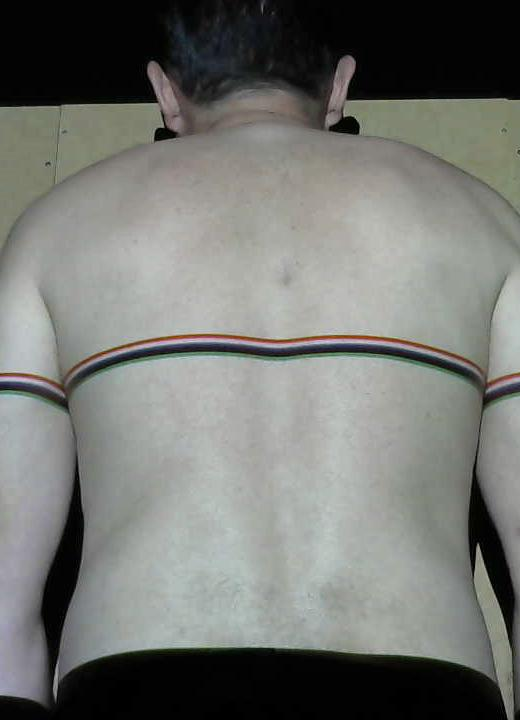
\includegraphics[width=\textwidth]{11_obj_color.jpg}
         \caption{Imagem $\mathbf{A}$ em RGB.}
         \label{fig:cordetect:rgb}
     \end{subfigure}
     \hfill
     \begin{subfigure}[b]{0.4\textwidth}
         \centering
         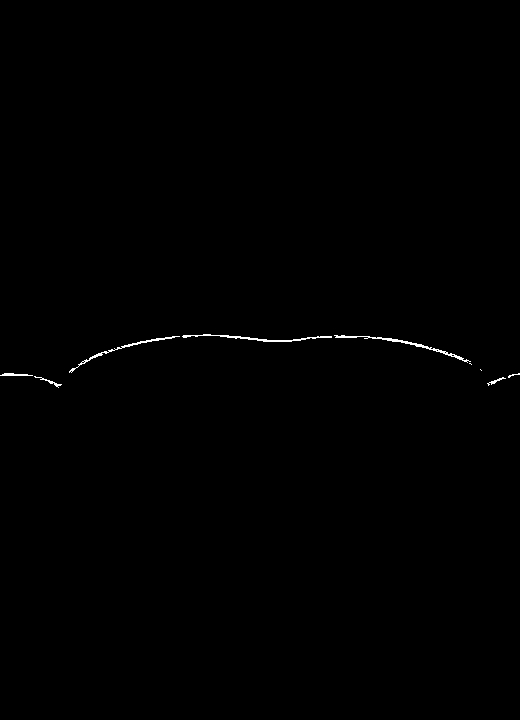
\includegraphics[width=\textwidth]{grayscale.jpg}
         \caption{Imagem $\mathbf{D}$ em BW.}
         \label{fig:cordetect:bw}
     \end{subfigure}
\caption{Detecção de cores.}
\label{fig:cordetect}
\end{figure}

Assim, para obter a linha detetada em branco e preto da Figura \ref{fig:cordetect:bw} 
a partir da linha projetada em cores da Figura \ref{fig:cordetect:rgb}, 
é utilizada a função $func\_compare()$, de modo que primeiro selecionamos um pixel $\mathbf{a}_c$ na imagem $\mathbf{A}$,
representando este pixel a cor a detetar, e logo comparamos
cada pixel $\mathbf{a}_l \in \mathbf{A}$, obtendo como resultado desta comparação $\mathbf{d}_l$, é dizer
\begin{equation}\label{eq:funccompare2}
\mathbf{d}_l\leftarrow func\_compare(\mathbf{a}_l,\mathbf{a}_c,\epsilon),\quad \forall~ 1\leq l\leq L,
\end{equation}
apos estes cálculos os valores $\mathbf{d}_l$ são ordenados para formar a imagem $\mathbf{D}$, 
como exemplifica a Figura \ref{fig:cordetect:bw}, onde a cor branca representa um 
valor $1$ e a cor preta um valor $0$.
No caso da Figura \ref{fig:cordetect} é usado o valor $\epsilon=0.25$.




\end{document}
